%%=============================================================================
%% Methodologie
%%=============================================================================

\chapter{\IfLanguageName{dutch}{Methodologie}{Methodology}}
\label{ch:methodologie}

%% TODO: Hoe ben je te werk gegaan? Verdeel je onderzoek in grote fasen, en
%% licht in elke fase toe welke stappen je gevolgd hebt. Verantwoord waarom je
%% op deze manier te werk gegaan bent. Je moet kunnen aantonen dat je de best
%% mogelijke manier toegepast hebt om een antwoord te vinden op de
%% onderzoeksvraag.

In de vorige hoofdstukken werden de frameworks die in deze studie vergeleken zullen worden geselecteerd en hun achtergrond besproken. In dit hoofdstuk wordt de effectieve vergelijking tussen de verschillende frameworks gemaakt. Verschillende belangrijke onderdelen van mobiele applicatieontwikkeling komen aan bod tijdens de vergelijking. Voor elk framework wordt eerst de aanpak op dit specifieke punt uitgelegd en vervolgens worden beide aanpakken met elkaar vergeleken. In deze vergelijking worden enkel React Native en Flutter met elkaar vergeleken, gezien er nog geen technische aspecten van .NET MAUI gekend zijn op het moment van schrijven.

\section{Vergelijking eigenschappen}
\label{sec:vglEigenschappen}

Elk framework heeft zijn eigen manier om bepaalde zaken aan te pakken. In deze sectie worden de verschillende aanpakken van de frameworks besproken op het gebied van navigatie, toegang tot de native API's, opbouwen van de gebruikersinterface van de applicatie en de styling van de applicatie.

\subsection{Navigatie binnen de applicatie}
\label{subsec:navigatieApplicatie}

Een belangrijk deel van elke applicatie is de mogelijkheid om te kunnen navigeren tussen verschillende pagina's van de applicatie. Elk cross-platform framework moet dus de mogelijkheid voorzien om de ontwikkelaar toe te staan deze functionaliteit te verwerken in de applicatie. Elk framework gaat hier op zijn eigen manier mee om. De aanpak van beide frameworks wordt uitgelegd in de volgende secties en vervolgens met elkaar vergeleken.

\subsubsection{React Native}
\label{subsubsec:navigatieReactNative}

React Native maakt voor de navigatie tussen de verschillende pagina's gebruik van een library genaamd React Native Navigation. Dit is een standalone library die de ontwikkelaar in staat stelt om zowel op Android als iOS navigatie aan te leveren die een native uitstraling heeft. Het is één van de vele populaire libraries binnen React Native die ontwikkeld zijn door de uitgebreide community achter React Native. Onderliggend maakt deze library ook gebruik van een andere library genaamd Animated om de animaties tijdens het navigeren naar een andere pagina aan te bieden. De animaties en gebaren die gepaard gaan met het navigeren kunnen volledig aangepast worden aan de voorkeuren van de ontwikkelaar. Er is dus zeer veel vrijheid en de gebruiker krijgt een applicatie die navigeert zoals een native applicatie. 

Om de navigatie te gebruiken moet de ontwikkelaar de hele applicatie wrappen in een navigatiecontainer. Op deze manier heeft de library toegang tot de gehele applicatie en kan de ontwikkelaar de navigatie tussen de verschillende pagina's instellen naar wens. De werkwijze om de applicatie te wrappen met de navigatiecontainer en de verschillende pagina's toe te voegen aan de navigatiestack is te zien in figuur \ref{fig:opzettenNavigatieReactNative}.

\begin{figure}
    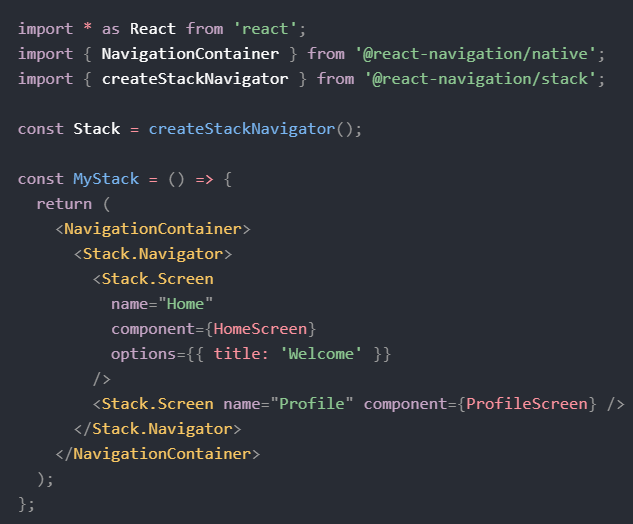
\includegraphics[width=\linewidth]{OpzettenNavigatieReactNative.png}
    \caption{Opzetten navigatie in een React Native applicatie. Bron: reactnative.dev/docs/navigation}
    \label{fig:opzettenNavigatieReactNative}
\end{figure}

Vervolgens moet er vastgelegd worden naar welke pagina er genavigeerd moet worden bij de uitvoering van een bepaald actie, zoals bv de klik op een bepaalde knop. Om dit mogelijk te maken krijgt elke component die een pagina voorstelt een attribuut navigation mee. In dit attribuut zitten methodes van de library die het navigeren tussen de verschillende pagina's mogelijk maakt. De opzet van een simpele navigatie is te zien in figuur \ref{fig:navigerenReactNative}. 

Zoals eerder vermeld heeft de library zeer veel mogelijkheden en levert het een navigatie af die native aanvoelt voor de gebruiker. Om dit te bereiken beschikt React Native Navigation ook over verschillende packages die o.a. tabs en drawer functionaliteit aanbieden. Dit zijn twee populaire manieren om te navigeren binnen een applicatie. Door dit aan te bieden in een package moet de ontwikkelaar niet helemaal zelf deze functionaliteit gaan uitwerken en wordt de standaard die de gebruiker gewoon is van native applicaties geëvenaard.

\begin{figure}
    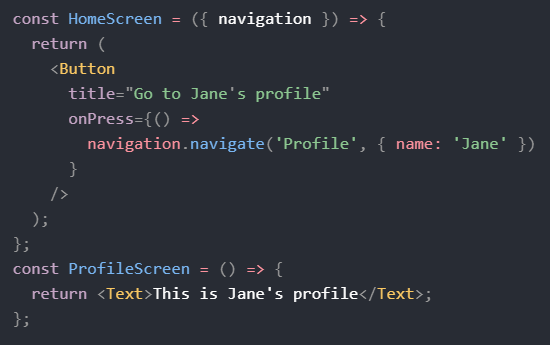
\includegraphics[width=\linewidth]{NavigerenPaginasReactNative.png}
    \caption{Navigeren naar een andere pagina in React Native. Bron: reactnative.dev/docs/navigation}
    \label{fig:navigerenReactNative}
\end{figure}

\subsubsection{Flutter}
\label{subsubsec:navigatieFlutter}

Flutter maakt voor de navigatie binnen een applicatie gebruik van de klasse Navigator. Deze klasse op zich is ook een widget, de bouwstenen waarmee een Flutter applicatie gebouwd wordt. In Flutter worden de verschillende pagina's en schermen van een applicatie routes genoemd. Deze routes worden op een stack geplaatst, die de volgorde van de routes bijhoudt. Er zijn twee verschillende aanpakken van navigatie binnen Flutter: de ene is gebaseerd op een vaste volgorde waar alle schermen elkaar opvolgen en de andere laat de ontwikkelaar toe om op aangepaste wijze te navigeren tussen verchillende pagina's. Beide aanpakken worden in de volgende paragrafen verder besproken. 

De eerste aanpak laat de gebruiker toe om in een vaste volgorde door de applicatie te navigeren. Dit is voornamelijk belangrijk als de gebruiker terug wil gaan naar het vorige scherm. In dit geval is het alleen maar logisch om naar de vorige route in de stack te gaan. Het is ook meteen de meest eenvoudige vorm van navigatie. Als de gebruiker naar een andere pagina navigeert wordt deze bovenaan de stack geplaatst. Indien de gebruiker terug wenst te gaan wordt de bovenste route terug verwijderd van de stack en komt de gebruiker op de vorige pagina terecht.

De tweede aanpak is een iets gecompliceerdere aanpak. Deze volgt geen logische volgorde maar wel de volgorde die vastgelegd is door de ontwikkelaar. De aanpak berust op een Navigator.pages object. Hieraan kunnen de verschillende pagina's toegevoegd worden. Vervolgens zal de Navigator dit Navigator.pages object omzetten in een stack van routes. Indien een nieuwe pagina wordt toegevoegd aan Navigator.pages dan wordt de stack ook geüpdate. 

Een applicatie kan uit zeer veel verschillende schermen bestaan. Om de navigatie ertussen overzichtelijk te houden voor de ontwikkelaar beschikt Flutter over een functie om de routes een naam te geven. Vervolgens kan de pagina aan de hand van zijn naam getoond worden. In figuur \ref{fig:namedRoutesFlutter} is de definitie van een map te zien die de naam van een route bevat en de builder die de route effectief zal tonen op het scherm. In figuur \ref{fig:useNamedRoutesFlutter} is te zien hoe de route effectief getoond kan worden. Uit de naam van de methode wordt duidelijk dat ook deze methode gebruik maakt van een stack voor de navigatie. De nieuwe route wordt bovenop de stack geplaatst.

Beide methodes maken dus gebruik van dezelfde stack en kunnen dus ook door elkaar gebruikt worden. Dit is een logische aanpak, aangezien een logische volgorde in een applicatie absoluut noodzakelijk is. Indien een gebruiker terug wil gaan is het alleen logisch om naar de vorige stap te gaan, ongeacht welke methode gebruikt werd om naar de huidige pagina te navigeren. 

Verder is het in Flutter mogelijk om een route een waarde te laten terug geven. Dit is bijvoorbeeld handig indien de gebruiker op oké moet klikken alvorens er naar het volgende scherm gegaan kan worden. Indien de gebruiker uit dit scherm gaat door de terug knop van het systeem te gebruiken is de waarde die teruggegeven wordt null en zal het volgende scherm dus niet getoond worden.

Tot slot geeft de Navigator klasse de ontwikkelaar ook de mogelijkheid om popups te tonen op het scherm? Dit zijn schermen die niet de volledig oppervlakte van het scherm in nemen en dus nog een deel van het onderliggende scherm tonen. Het onderliggende scherm wordt echter geblokkeerd, de gebruiker kan dus enkel binnen de popup input geven. Deze popups gedragen zich verder als een normale route, de navigatie naar een popup en er weg van is dus exact hetzelfde.

\begin{figure}
    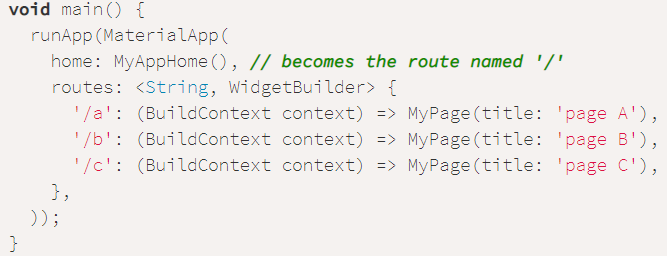
\includegraphics[width=\linewidth]{NamedRoutesFlutter.png}
    \caption{Opzetten navigatie met benoemde routes in Flutter. Bron: \textcite{Flutter.dev2020}}
    \label{fig:namedRoutesFlutter}
\end{figure}

\begin{figure}
    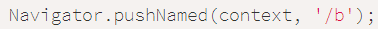
\includegraphics[width=0.5\linewidth]{UseNamedRouteFlutter.png}
    \caption{Benoemde route tonen in Flutter. Bron: \textcite{Flutter.dev2020}}
    \label{fig:useNamedRoutesFlutter}
\end{figure}



